%\addbibresource{/home/jorgsk/Dropbox/phdproject/bibtex/jorgsk.bib}
\subsection{Model of initial transcription}
Our goal was to construct an accuarte kinetic model of initial transcription
that is able to be compared with availabe literature. To this end, it is
necessary that the computational model is highly descriptive of the process.
To do so, we decided to construct our model using experimentally measured
abortive profiles (the abortive probability at different ITS positions), which
we use to obtain the rate of backtracking at each ITS position. This is likely
to result in a highly accurate model of initial transcription, since
unscrunching and abortive RNA release are rate limiting for initial
transcription \cite{revyakin_abortive_2006}. Specifically, we assume in our
model that each backtracking event during initial transcription will result in
an abortive RNA with similar rates for all ITS positions. With this
assumption, we can use, for a given rate of NAC, the experimentally obtained
abortive probability (AP)~\cite{hsu_quantitative_1996} to calculate the rate
of backtracking at each ITS position:
\begin{equation*}
    b = \frac{NAC\cdot AP}{1-AP},
\end{equation*}

We model intitial transcription using the kinetic scheme given in Figure
\ref{fig:model}. The abortive probabilities for all simulations are obtained
from Hsu et. al \cite{hsu_initial_2006}.
Figure~\ref{fig:parameter_estimation}A shows the initial transcription kinetic
scheme together with placeholder values for the the estimated rates.
Figure~\ref{fig:parameter_estimation}B shows example values obtained for the
N25 promoter when using $NAC=10/s$. The rate of FL product synthesis upon
promoter escape is given by $NAC/d$ where d is the number of nts from promoter
escape until runoff.

\subsection{Implementation and parameter estimation for N25}
To solve the kinetic scheme we use the direct method of the stochastic
simmulation algorithm \cite{gillespie_exact_1977} as implemented in the StocPY
software \cite{maarleveld_stochpy:_2013}. By using stochastic simulations, we
are able to simulate transcription to the level of single RNA polymerases,
which includes the stochastisity the follows with low copy-number reactions.
In this way, we are able to compare and fit the model to single-molecule
experiments of initial transcription.

We estimate the rate constants of NAC, promoter escape, and unscrunching using an
iterative heuristic process. In the first iteration, we sample 1000 times
values for the three rate constants in the range 1/s to 25/s. For each sample,
we use the NAC value to obtain rate constants for backtracking (as illustrated
in Figure~\ref{fig:parameter_estimation}). We then simulate initial
transcription on N25 with 100 RNAPs (the number of single-RNAP transcription
events in Revyakin et.\ al \cite{revyakin_abortive_2006}), and find the
cumulative distrivution of time spent in abortive cycling, which is compared
to the measured value using a root mean squared distance. After all 1000
simulations are finished, we rank them by score and calculate the weighted
mean and weighted standard deviation of the top 20 samples, using the scores
as weights. For the next iteration, we again sample 1000 random values, but
this time the boundaries for the three rate constants are given by the
weighted mean $\pm$ the weighted standard deviation as computed for the
previious iteration. We repeat this iterative process until the average score
of the top 20 results has reaches within 5\% of that of the previous iteration.

\begin{figure}
	\begin{center}
        \includegraphics{../illustrations/model.pdf}
	\end{center}
    \caption{Kinetic model scheme. From the open complex (OC)
    transcroption proceeds in cycles of nucleotide additions from one initial
    transcribing complex (IC) to the next, where each IC is identified by the
    length of the nascent RNA. For ICs with an 2nt RNA or more, there is a
    competition between the nucleotide addition cycle (NAC) and backtracking.
    Backtracking leads to a backtracked state from which unscrunching and
    abortive RNA release occurs.}
    \label{fig:model}
\end{figure}

\begin{figure}
	\begin{center}
        \includegraphics{../illustrations/parameter_estimation.pdf}
	\end{center}
    \caption{Estimated rates. NAC ($x$), promoter escape ($y$), and
    unscrunching and abortive release ($z$), and the backtracking rates
    $b_i(x)$ are estimated}
    \label{fig:parameter_estimation}
\end{figure}
%\bibliography{/home/jorgsk/Dropbox/phdproject/bibtex/jorgsk}
